%%%%%%%%%%%%%%%
%
% $Autor: Wings $
% $Datum: 2020-01-29 07:55:27Z $
% $Pfad: General/I2C.tex
% $Version: 1785 $
%
%
%%%%%%%%%%%%%%%

\chapter{Protokoll I\textsuperscript{2}C}


 
Die Firma Philips führte Anfang der 1980er Jahre eine neue serielle Zweidraht-Kommunikationsstandard ein, den \textit{Inter-Integrated-Circuit Bus}, kurz I2C oder I\textsuperscript{2}C. Die Datenübertragung findet über eine Leitung statt, die \ac{sda} Leitung. Über \ac{scl} wird ein Taktsignal vorgegeben. Die Taktfrequenz liegt zwischen 100 kHz (Standard-Mode) bis 400 kHz (Speed-Mode). 

Der erste Schritt zur Datenübertragung in diesem Protokoll ist die Startbedingung. Der Master übermittelt eine Bausteinadresse an den Slave, siehe Abbildung \ref{fig:I2C-Aufbau}\cite{Gehrke:2022}. Der Master wird im Protokoll I\textsuperscript{2}C durch die Code-Zeile \PYTHON{Wire.begin();} definiert. Durch das Weglassen einer Adresse innerhalb der Klammern, wird der Arduino als Master initialisiert\cite{ArduinoWire:2022}.

\begin{figure}[H] 
    \centering 
    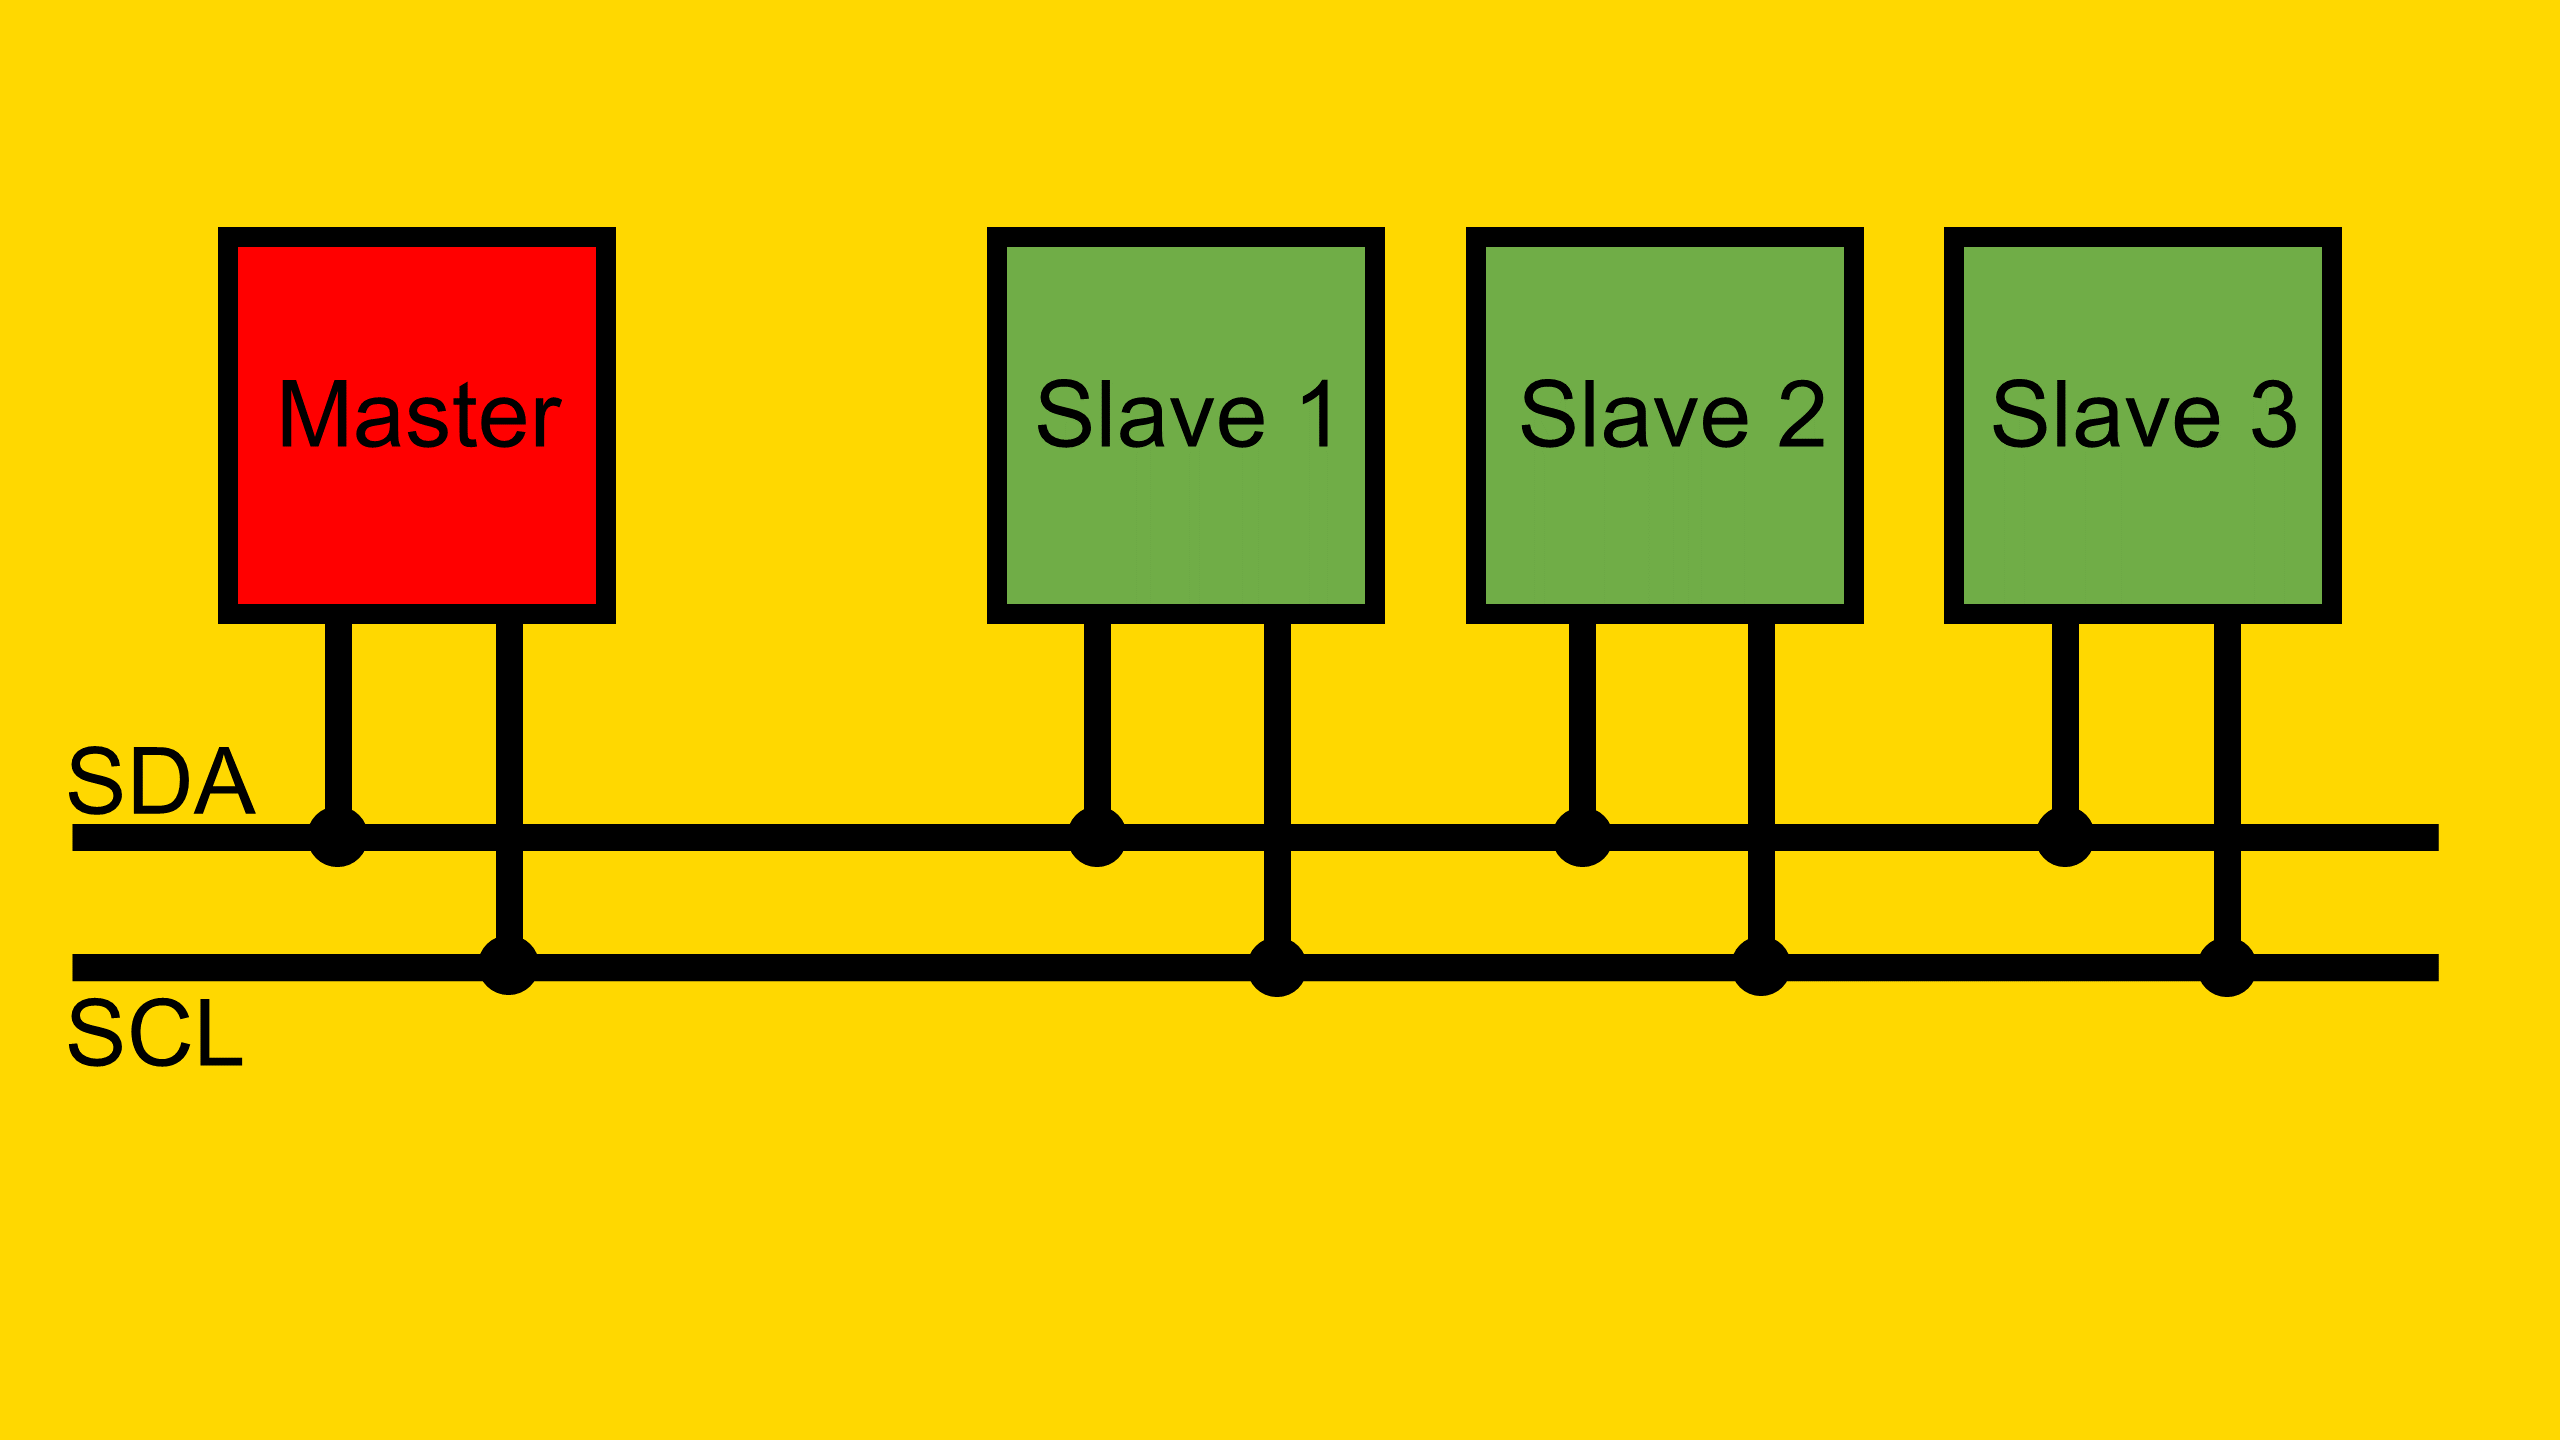
\includegraphics[width=10cm]{I2C/I2C}
    \caption[Aufbau des Protokolls I\textsuperscript{2}C]{Aufbau des Protokolls I\textsuperscript{2}C \cite{Gehrke:2022}}
    \label{fig:I2C-Aufbau}
\end{figure}
\Mynote{Grafik besser mit tikz}

Ist diese gesendete Bausteinadresse identisch mit der Adresse des Slaves, \Mynote{unverständlich; Beispiel fehlt} kann der Slave an der Kommunikation mit dem Master teilnehmen. So können auch mehrere Slaves angesprochen werden. Im nächsten Schritt wird ein einzelnes Bit gesendet mit dem angezeigt wird, ob der Master vom Slave Daten lesen möchte (1:Lesen/Read) oder Daten an den Slave übermitteln möchte (0:Schreiben/Write). Im Anschluss werden dann die Daten an den Slave gesendet bzw. vom Master empfangen. Dieser Datenaustausch wird dann bestätigt und weitere Daten können ausgetauscht werden. Soll die Kommunikation beendet werden wird eine Stopp-Bedingung gesendet, siehe Abbildung \ref{fig:I2C-Protokoll}. \cite{Gehrke:2022}  

\begin{figure}[H] 
    \centering 
    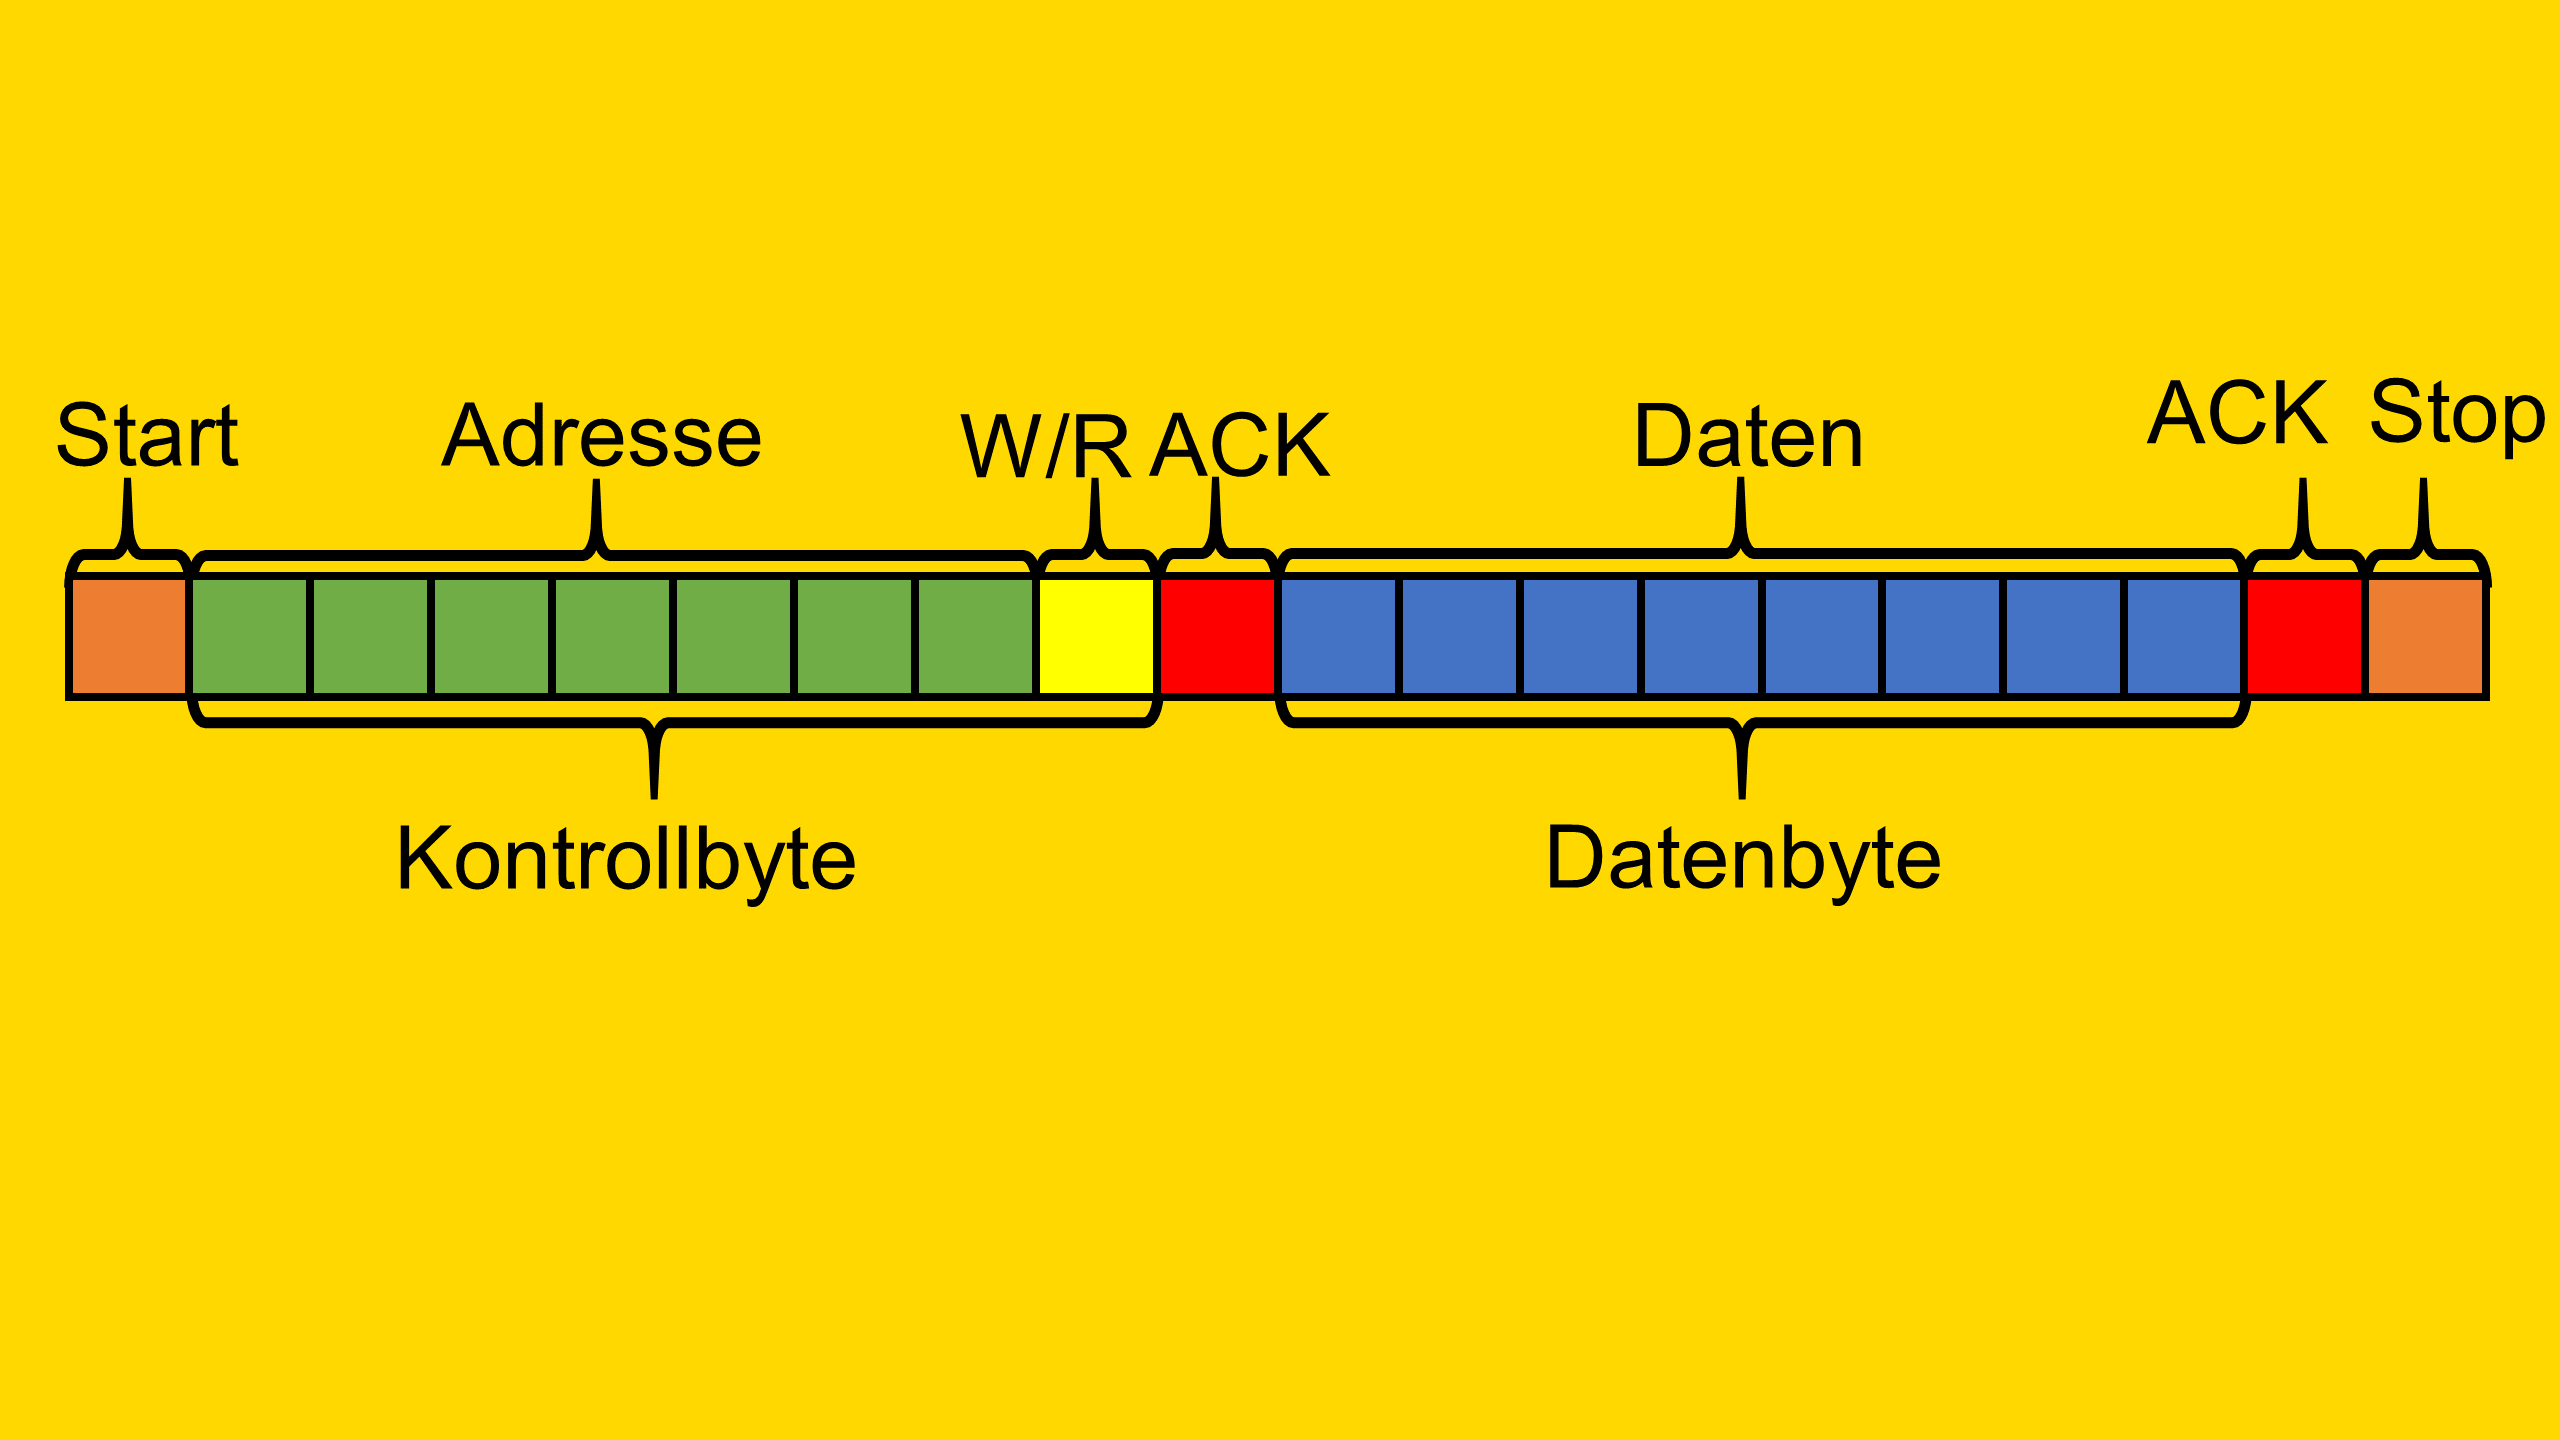
\includegraphics[width=10cm]{I2C/I2CProtocol}
    \caption{I2C-Protokoll Quelle: \cite{Gehrke:2022}}
    \label{fig:I2C-Protokoll}
\end{figure}
\Mynote{Grafik besser mit tikz}


Das Protokoll wird auch bei der Verwendung  interner Sensoren, wie zum Beispiel des Sensors APDS-9960, benutzt. Ebenfalls die Anbindung eines OLED-Displays erfolgt über I\textsuperscript{2}C.


\section{Pin-Belegung für I\textsuperscript{2}C beim Arduino Nano 33 BLE Sense}

Der Arduino Nanao 33 BLE Sense nutzt zur Realisierung den Pin A4 als Datenleitung SDA und Pin A5 als Taktleitung SCL. 


Einige Sensoren sind per Inter-Integrated-Circuit, auch I2C genannt, mit
dem Arduino vernetzt. Die Schnittstelle besteht aus einer Daten- und ei-
ner Taktleitung, weshalb die Daten auch über längere Strecken übertra-
gen werden können als beispielsweise von der SPI-Schnittstelle. Aufgrund
der zwei benötigten Leitungen wird der I2C auch als TWI (Two Wire)
Schnittstelle bezeichnet. Alle zu übertragenden Daten werden nach dem
FIFO-Prinzip/ seriell hintereinander gesendet. Der Arduino ist beim I2C
der Master und die Sensoren sind die Slaves.[Meroth2021]
Master und Slave sind jeweils über SDA und SCL Leitung verbunden. Die
SDA (Serial Data) Leitung arbeitet in beide Richtungen, also bidirektio-
nal, und ist für den Datenaustausch zuständig. Die SCL (Serial Clock)
Leitung sendet die Taktimpulse, welcher bei allen Teilnehmern synchron
abläuft. Kommuniziert wird mit 128 Teilnehmern, bei einem Arduino
können also noch 127 Sensoren am Bus angeschlossen werden.[I2C]

\begin{figure}[!ht]
    \centering
    \resizebox{1\textwidth}{!}{%
        \begin{circuitikz}
            \tikzstyle{every node}=[font=\normalsize]
            \draw [dashed] (1.5,3) -- (20,3);
            \draw [short] (1.5,0) -- (20,0);
            \draw [short] (1.5,-0.5) -- (20,-0.5);
            %\draw (14.25,3) to[R] (14.25,-0.5);
            %\draw (13.25,3) to[R] (13.25,0);
            % Draw rectangular resistors
            \draw (14.1,0.5) rectangle (14.4,1.5);
            \draw (13.1,0.8) rectangle (13.4,1.8);
            
            \draw (14.25,0.5) -- (14.25,-0.5);
            \draw (14.25,1.5) -- (14.25,3);
            
            \draw (13.25,0.8) -- (13.25,0);
            \draw (13.25,1.8) -- (13.25,3);
            
            \node [font=\normalsize, align=center] at (16.25,1.5) {pull-up \\ resistors};
            \node [font=\normalsize] at (0.75,3) {Vs};
            \node [font=\normalsize] at (0.75,0.25) {SDA};
            \node [font=\normalsize] at (0.75,-0.75) {SCL};
        \end{circuitikz}
    }%
    %\caption{I2C}
\end{figure}



\begin{figure}[!ht]
    \centering
    \resizebox{1\textwidth}{!}{%
        \begin{circuitikz}
            \tikzstyle{every node}=[font=\large]
            \draw [ black , line width=0.5pt](1.25,11.25) to[short] (20.75,11.25);
            \draw [ gray!70, , line width=3pt](1.25,12.25) to[short] (20.75,12.25);
            \draw [ black, line width=0.5pt, dashed] (1.25,15) -- (20.75,15);
            %\draw [ color={rgb,255:red,115; green,115; blue,115} , line width=0.5pt](14.5,15) to[R] (14.5,12.25);
            %\draw [ color={rgb,255:red,115; green,115; blue,115} , line width=0.5pt](15.75,15) to[R] (15.75,11.25);
            %Resistors
            \draw (14.1,13.3) rectangle (14.4,14.3);
            \draw (13.1,13.4) rectangle (13.4,14.4);
            
            \draw (14.25,15) -- (14.25,14.3);
            \draw (14.25,13.3) -- (14.25,11.25);
            
            \draw (13.25,15) -- (13.25,14.4);
            \draw (13.25,13.4) -- (13.25,12.25);
            
            \node [font=\large, black] at (17.75,13.75) {\textbf{pull-up}};
            \node [font=\large, black] at (17.75,13) {\textbf{resistors}};
            \node [font=\large, black] at (0.75,15) {Vs};
            \node [font=\large, black] at (0.5,12.5) {SDA};
            \node [font=\large, black] at (0.5,11.25) {SCL};
            \draw [ color={rgb,255:red,97; green,97; blue,97} , fill={rgb,255:red,97; green,97; blue,97}, line width=0.5pt ] (3.25,12.25) circle (0.25cm);
            \draw [ color={rgb,255:red,97; green,97; blue,97} , fill={rgb,255:red,97; green,97; blue,97}, line width=0.5pt ] (4.75,11.25) circle (0.25cm);
            \draw [ color={rgb,255:red,97; green,97; blue,97} , fill={rgb,255:red,97; green,97; blue,97}, line width=0.5pt ] (10.5,12.25) circle (0.25cm);
            \draw [ color={rgb,255:red,97; green,97; blue,97} , fill={rgb,255:red,97; green,97; blue,97}, line width=0.5pt ] (12,11.25) circle (0.25cm);
            \draw [ color={rgb,255:red,97; green,97; blue,97} , fill={rgb,255:red,97; green,97; blue,97}, line width=0.5pt ] (17.5,12.25) circle (0.25cm);
            \draw [ color={rgb,255:red,97; green,97; blue,97} , fill={rgb,255:red,97; green,97; blue,97}, line width=0.5pt ] (19,11.25) circle (0.25cm);
            \draw [ color={rgb,255:red,97; green,97; blue,97} , fill={rgb,255:red,97; green,97; blue,97}, line width=0.5pt ] (1.5,8.75) rectangle (6.25,5.75);
            \draw [ color={rgb,255:red,237; green,237; blue,237} , fill={rgb,255:red,237; green,237; blue,237}, line width=0.5pt ] (8.75,8.75) rectangle (13.5,5.5);
            \draw [ color={rgb,255:red,237; green,237; blue,237} , fill={rgb,255:red,237; green,237; blue,237}, line width=0.5pt ] (15.75,9) rectangle (20.5,5.75);
            \draw [, line width=0.5pt](4.75,11) to[short] (4.75,8.75);
            \draw [, line width=0.5pt](3.25,12) to[short] (3.25,8.75);
            \draw [, line width=0.5pt](12,11) to[short] (12,8.75);
            \draw [, line width=0.5pt](10.5,12) to[short] (10.5,8.75);
            \draw [, line width=0.5pt](19,11) to[short] (19,9);
            \draw [, line width=0.5pt](17.5,12) to[short] (17.5,9);
            \node [font=\huge] at (11.25,7.25) {son x};
            \node [font=\huge] at (18,7.25) {son y};
            \node [font=\huge, color={rgb,255:red,245; green,245; blue,245}] at (3.75,7.25) {mother};
            \node [font=\LARGE] at (12,3.5) {\textbf{set address to son of interest}};
        \end{circuitikz}
    }%
    %\caption{I2C2}
\end{figure}


\begin{figure}[!ht]
    \centering
    \resizebox{1\textwidth}{!}{%
        \begin{circuitikz}
            \tikzstyle{every node}=[font=\large]
            \draw [ black , line width=0.5pt](1.25,11.25) to[short] (20.75,11.25);
            \draw [ gray!70, , line width=3pt](1.25,12.25) to[short] (20.75,12.25);
            \draw [ black, line width=0.5pt, dashed] (1.25,15) -- (20.75,15);
            %\draw [ color={rgb,255:red,115; green,115; blue,115} , line width=0.5pt](16,15) to[R] (16,12.25);
            %\draw [ color={rgb,255:red,115; green,115; blue,115} , line width=0.5pt](16.75,15) to[R] (16.75,11.25);
            
            %Resistors
            \draw (15.85,13.3) rectangle (16.15,14.3);
            \draw (16.6,13.4) rectangle (16.9,14.4);
            
            \draw (16,15) -- (16,14.3);
            \draw (16.75,13.4) -- (16.75,11.25);
            
            \draw (16.75,15) -- (16.75,14.4);
            \draw (16,13.3) -- (16,12.25);
            
            
            \node [font=\large, black] at (18,13.75) {\textbf{pull-up}};
            \node [font=\large, black] at (18,13) {\textbf{resistors}};
            \node [font=\large, black] at (0.75,15) {Vs};
            \node [font=\large, black] at (0.5,12.5) {SDA};
            \node [font=\large, black] at (0.5,11.25) {SCL};
            \draw [ gray, fill=gray, line width=0.5pt ] (3.25,12.25) circle (0.25cm);
            \draw [ gray, fill=gray, line width=0.5pt ] (4.75,11.25) circle (0.25cm);
            \draw [ gray, fill=gray, line width=0.5pt ] (9,12.25) circle (0.25cm);
            \draw [ gray, fill=gray, line width=0.5pt ] (10.5,11.25) circle (0.25cm);
            \draw [ gray, fill=gray, line width=0.5pt ] (14.25,12.25) circle (0.25cm);
            \draw [ gray, fill=gray, line width=0.5pt ] (15.75,11.25) circle (0.25cm);
            \draw [ gray, fill=gray, line width=0.5pt ] (1.5,8.75) rectangle (6.25,5.75);
            \draw [color={rgb,255:red,247; green,247; blue,247} , fill={rgb,255:red,247; green,247; blue,247}, line width=0.5pt ] (7.25,8.75) rectangle (12,5.5);
            \draw [ color={rgb,255:red,247; green,247; blue,247} , fill={rgb,255:red,247; green,247; blue,247}, line width=0.5pt ] (12.75,8.75) rectangle (17.5,5.);
            \draw [, line width=0.5pt](4.75,11) to[short] (4.75,8.75);
            \draw [, line width=0.5pt](3.25,12) to[short] (3.25,8.75);
            \draw [, line width=0.5pt](10.5,11) to[short] (10.5,8.75);
            \draw [, line width=0.5pt](9,12) to[short] (9,8.75);
            \draw [, line width=0.5pt](14.25,12) to[short] (14.25,8.75);
            \draw [, line width=0.5pt](15.75,11) to[short] (15.75,8.75);
            
            
            \node [inner sep=0pt] at (3.75,7.25) {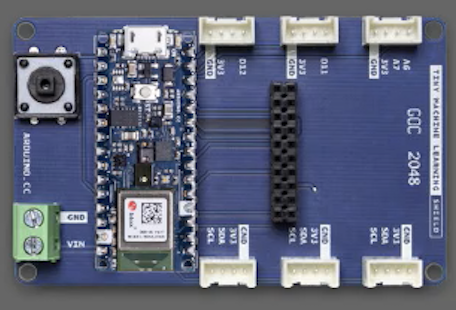
\includegraphics[width=3cm]{I2C/I2C31}};
            \node [inner sep=0pt] at (9.5,7.25) {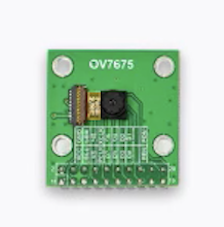
\includegraphics[width=3cm]{I2C/I2C32}};
            \node [inner sep=0pt] at (15,7.25) {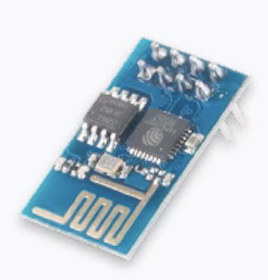
\includegraphics[width=3cm]{I2C/I2C33}};
            
            \node [font=\LARGE] at (12,3.5) {\textbf{set address to son of interest}};
        \end{circuitikz}
    }%
    %\caption{I2C3}
\end{figure}


\begin{tikzpicture}
    % I2C communication blocks
    % \definecolor{orange}{RGB}{255,200,0}
    
    \node[rectangle, fill=green, minimum width=1cm, minimum height=1cm] (start) {\textcolor{white}{START}};
    \node[rectangle, fill=orange, right=0cm of start, minimum width=3cm, minimum height=1cm] (address) {\textcolor{white}{ADDRESS}};
    \node[rectangle, fill=gray!20, right=0cm of address, minimum width=1cm, minimum height=1cm] (rw) {R/W};
    \node[rectangle, fill=blue, right=0cm of rw, minimum width=1cm, minimum height=1cm] (ack1) {\textcolor{white}{ACK}};
    \node[rectangle, fill=gray!60, right=0cm of ack1, minimum width=2cm, minimum height=1cm] (data) {\textcolor{white}{DATA}};
    \node[rectangle, fill=blue, right=0cm of data, minimum width=1cm, minimum height=1cm] (ack2) {\textcolor{white}{ACK}};
    \node[rectangle, fill=gray!60, right=0cm of ack2, minimum width=2cm, minimum height=1cm] (data2) {\textcolor{white}{DATA}};
    \node[rectangle, fill=blue, right=0cm of data2, minimum width=1cm, minimum height=1cm] (ack3) {\textcolor{white}{ACK}};
    \node[rectangle, fill=red, right=0cm of ack3, minimum width=1cm, minimum height=1cm] (stop) {\textcolor{white}{STOP}};
    
    % Rectangles
    \draw[green, fill=green] (0.5,-4) rectangle (1,-2.5);
    \node[green, below] at (0.75, -4) {START};
    
    \draw[orange, fill=orange] (3.5,-4) rectangle (4,-2.5);
    \node[orange, below] at (3.75, -4) {A$_1$};
    
    \draw[orange, fill=orange] (5.3,-4) rectangle (5.8,-2.5);
    \node[orange, below] at (5.55, -4) {A$_2$};
    
    \draw[orange, fill=orange] (9,-4) rectangle (9.5,-2.5);
    \node[orange, below] at (9.25, -4) {A$_N$};
    
    \draw[red, fill=red] (11.8,-4) rectangle (12.3,-2.5);
    \node[red, below] at (12.05, -4) {STOP};
    
    % Lines
    \draw[black, line width=1pt,dotted] (0.1,-2.7) -- (0.3,-2.7);
    \draw[black, line width=1pt] (0.3,-2.7) -- (0.6,-2.7) -- (0.8,-3) -- (2.5,-3) -- (2.7,-2.7) -- (4.4,-2.7) -- (4.6,-3) -- (6.3,-3) -- (6.5,-2.7)-- (7.2,-2.7);
    \draw[black, line width=1pt] (7.7,-2.7)-- (8.2,-2.7) -- (8.4,-3) -- (10.1,-3) -- (10.3,-2.7);
    \draw[black, line width=1pt,dotted] (7.2,-2.7) -- (7.7,-2.7);
    \node[black, below, font=\tiny] at (0, -2.6) {SDA};
    
    
    \draw[black, line width=1pt] (2.6,-2.75) -- (2.7,-3) -- (4.4,-3) -- (4.6,-2.7) -- (6.3,-2.7) -- (6.5,-3) -- (7.2,-3);
    \draw[black, line width=1pt] (7.7,-3)-- (8.2,-3) -- (8.4,-2.7) -- (10.1,-2.7) -- (10.3,-3) -- (12,-3) -- (12.2,-2.7) -- (12.5,-2.7);
    \draw[black, line width=1pt,dotted] (7.2,-3) -- (7.7,-3);
    
    \draw[black, line width=1pt] 
    (0.3,-3.4) -- (2,-3.4) -- (2.2,-3.8) -- (3,-3.8) -- (3.2,-3.4) -- 
    (4,-3.4) -- (4.2,-3.8) -- (5,-3.8) -- (5.2,-3.4) -- (6,-3.4) -- 
    (6.2,-3.8) -- (7,-3.8) -- (7.2,-3.4);
    \draw[black, line width=1pt] (7.7,-3.4) -- (8,-3.4)-- (8.2,-3.8) -- 
    (9,-3.8) -- (9.2,-3.4) -- (10,-3.4) -- (10.2,-3.8) -- (11,-3.8) -- 
    (11.2,-3.4) -- (13,-3.4);
    \draw[black, line width=1pt,dotted] (7.2,-3.4) -- (7.7,-3.4);
    \node[black, below, font=\tiny] at (0, -3.5) {SCL};
    
    %Dotted lines
    \draw[black, line width=1pt,dotted] (12.5,-2.7) -- (12.9,-2.7);
    
    
    
    
\end{tikzpicture}
%\end{document}